\documentclass[10pt,a4paper]{article}
\usepackage[utf8]{inputenc}
%\usepackage[french]{babel}
\usepackage[T1]{fontenc}
\usepackage{amsmath}
\usepackage{amsfonts}
\usepackage{amssymb}
\usepackage{verbatim}
\usepackage{graphicx}

\author{Donatien Dallery}
\title{La télédétection et GéoBretagne : méthodes, produits et analyses}
\begin{document}
\maketitle

\begin{abstract}
GéoBretagne a décidé d'intégrer des données de télédétection à son catalogue. Dans un premier temps, 4 produits sont disponibles : 
\begin{itemize}
\item le NDVI pour la distinction des surfaces végétales/non végétales
\item l'Evaporative Fraction pour estimer l'évaporation d'un sol et donc, son potentiel hydrique
\item les températures moyenne sur 8 jours de jour, comme de nuit
\end{itemize}
Chacun de ces produits possède une dimension temporelle afin de suivre l'évolution de ces indices de manière intra et inter-annuelle. Le capteur MODIS a été choisi pour effectuer cette introduction à la télédétection.
\end{abstract}

\section{Introduction}

La définition officielle de la télédétection est « l’ensemble des connaissances et techniques utilisées pour déterminer des caractéristiques physiques et biologiques d’objets par des mesures effectuées à distance, sans contact matériel avec ceux-ci » (COMITAAS, 1988).\smallbreak

La notion de "sans contact matériel avec ceux-ci" correspond à l'acquisition d'informations sur la Terre à partir de satellites, avions, drones ou simplement d'un appareil photo jeté en l'air (à vos risques et périls). Pour l'étude d'autres planètes, les télescopes effectuent également de la télédétection étant donné qu'ils ne sont pas en contact avec celles-ci.\smallbreak

L'acquisition d'informations s'opère par la mesure du  spectre électromagnétiques dans différents domaines (figure \ref{spectreElectro}) :
\begin{itemize}
\item dans le visible pour l'oeil humain, comme un appareil photo
\item dans l'invisible pour l'oeil humain :
\begin{itemize}
\item l'infrarouge (télécommande, capteur thermique)
\item les micro-ondes (téléphone, radar)
\end{itemize}
\end{itemize}

\begin{figure}[!h]
\centering
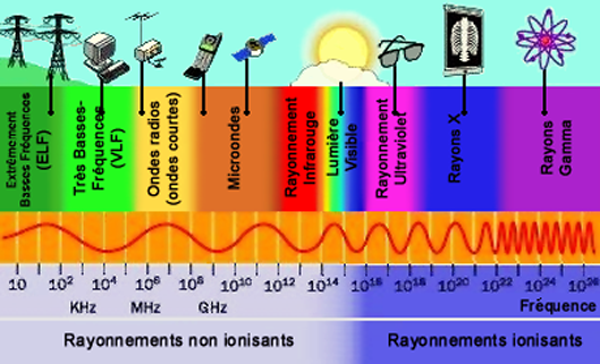
\includegraphics[scale=0.6]{img/spectre-electromagnetique.png}
\caption{Représentation du spectre électromagnétique (source : astronoo.com)}
\label{spectreElectro}
\end{figure}

Dans le cadre de cette introduction à la télédétection, les données employées se situent dans les domaines du visible et de l'invisible (infrarouge) et proviennent du capteur MODIS.

\subsection{Capteur MODIS}

Le capteur MODIS est un spectroradiomètre imageur (un appareil appareil photo) se trouvant sur deux satellites (Terra et Aqua) (figure \ref{modis}) mis en service par la NASA dont les données sont diffusées par l'United States Geological Survey (USGS) .

\begin{figure}[!h]
\centering
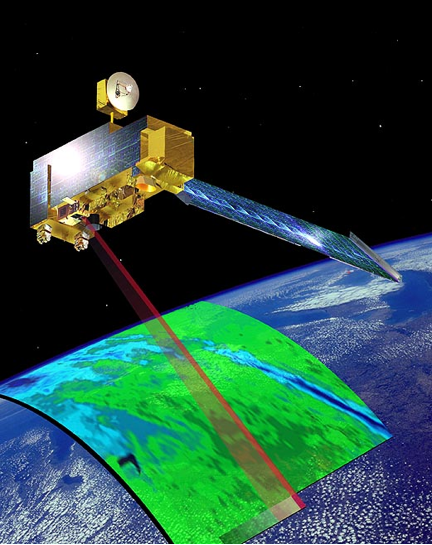
\includegraphics[scale=0.5]{img/modis.png}
\caption{Représentation du satellite Terra avec le capteur MODIS}
\label{modis}
\end{figure}

Ce capteur dispose d'une résolution spatiale allant de 250 mètres à 1 kilomètre avec une résolution temporelle journalière (vers 10h00). Une image de ce capteur couvre 2330 km$^2$ (figure \ref{modisGrid}).

\begin{figure}[!h]
\centering
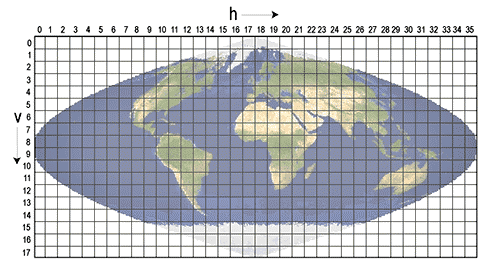
\includegraphics[scale=0.7]{img/modisGrid.png}
\caption{Grille d'acquisition des images MODIS}
\label{modisGrid}
\end{figure}

\subsection{Plan de travail}
\begin{itemize}
\item Téléchargement et stockage automatique des images MODIS (bandes + TempJour et TempNuit S8)
\item Calcul du NDVI, bord chaud/froid via nuage de points, récupérer 5\% min et max pour calculer EF
\item Remplir une fiche de métadonnées
\item Présenter le résultat
\end{itemize}

\section{Méthodologie}

La méthodologie correspond à une chaîne de traitement développée en Python.

\subsection{Téléchargement des données MODIS}

\begin{itemize}
\item Les données MODIS se situent sur le site :\newline \verb!https://lpdaac.usgs.gov/data_access/data_pool.!
\item Pour la Bretagne, il faut télécharger la tuile h17v04. 
\item Le capteur MODIS Terra va être celui qui sera utilisé pour calculer le NDVI (J. Wang et al., 2007) et aussi pour les autres informations.
\item Pour les températures jour/nuit S8 à 1km, le produit est MOD11A2 avec les produits LST day et night (température en Kelvin) avec un scale factor de 0.02.
\item Les bandes Red et Nir MODIS sont disponibles via le produit MOD09Q1 S8 à 250m avec un scale factor de 0.0001.
\end{itemize}  

La nomenclature des noms de fichiers est la suivante :
\begin{itemize}
\item MYD11A2.AYYYYDDD.hHHvVV.CCC.YYYYDDDHHMMSS.hdf
\begin{itemize}
\item YYYYDDD = Year and Day of Year of acquisition
\item hHH = Horizontal tile number (0-35)
\item vVV = Vertical tile number (0-17)
\item CCC = Collection number
\item YYYYDDDHHMMSS = Production Date and Time
\end{itemize}
\end{itemize}

L'évapotranspiration est disponible dans les données MODIS (MOD16A2) calculé selon cette méthode (http://www.ntsg.umt.edu/project/mod16).

\begin{enumerate}
\item Lancement du script (-path pour le répertoire où sauvegarder les données, -netrc pour indiquer le fichier contenant les identifiants pour télécharger les images, -fdate pour indiquer la date à partir de laquelle on souhaite télécharger les images, -ldate pour indiquer la date de fin de recherche des images).
\item Liste toutes les dates entre celle indiqué en paramètre et la date du jour.
\item Initialise l'url pour télécharger les données.
\item Se place au niveau de l'url et liste tous les liens à télécharger.
\item Télécharge les images qui ne l'ont pas encore été.
\end{enumerate}

Concernant une perspective, il serait intéressant de donner des intervalles de temps et non pas une date de départ.

\subsection{Calcul de l'Evaporative Fraction (EF)}

Lors de cette étape, nous disposons des bandes du rouge et du proche infrarouge, mais aussi des températures de jour et de nuit en Kelvin.

\begin{enumerate}
\item Liste tous les fichiers téléchargés.
\item  Pour chaque fichier, converti le type .hdf vers .GeoTiff et rééchantillonne les températures à la résolution spatiale des bandes du rouge et proche infrarouge (1km vers 250m).
\item Utilisation d'un shapefile de la région Bretonne pour découper la tuile MODIS et masquer les valeurs aberrantes de la mer.
\item Calcule le NDVI et supprime les valeurs <0 et >1 (valeurs aberrantes se situant dans la mer et qui ne peuvent être masquée sans rogner sur le territoire).
\item Calcul du FVC via le NDVI.
\item Supprime les pixels sans données (Nan) sur les images (si un pixel est Nan sur une image, supprime le même pixel sur l'autre) et calcule Tj-Tn.
\item Assigne une valeur Nan au FVC aux endroits où il n'y a pas de données sur Tj-Tn.
\item Génère un nuage de points pour employer la méthode de Priestley-Taylor pour déterminer EF par l'utilisation d'une équation de droite selon les bords sec et humide.
\item Génère les droites de régression et détermine l'équation pour calculer EF pour chacun des points.
\item Calcule EF et génère une image selon cette donnée.
\end{enumerate}

\section{Réunion 16/06/2017 (Donatien, Hervé, Fabrice)}
\begin{itemize}
\item Fait : Estimer coût mémoire (stockage) 4mo par date pour résolution 250m et 1mo pour résolution 1km et temps de téléchargement et calcul des données.
\item Fait : Conserver les données brutes et les diffuser également
\item Fait : Compression "deflate" à ajouter
\item Fait : Publier les bandes brutes decoupee/reechant/compress et les produits calculés.
\item Fait : Coverage view -> vue sur le geoserver où l'on indique différents rasters (Donnees brutes + EF)
\item Fait : Zone sans données -> on conserve les zones sans données pour le moment (solution avec interpolation pour recréer via la série temporelle ou faire des synthèse de 16j voir plus ?)
\item Entre deux images (dates), quelle est la pertinence d'une valeur identique entre ces deux dates (déduction qu'il ne s'est rien passé ou pas de temps trop faible pour le voir ?)
\item Pour présenter les valeurs EF, faire un découpage par zones pour donner les valeurs, courbes, etc... par zones et non pas à l'échelle du pixel.
\item Organigramme -> traitement en verticale et publication vers la droite.
\item Fait : Publier sur GeoSas des donnees.
\item Creer un GeoRss + mail + tweet + page html avec lien direct pour animation, donnees pour informer sur de la publication de donnees + lien vers mviewer.
\item Geoxxx pour traitement et mise au point (temps telechargement, traitement, demo) et geoserver pour publication (Geowww) via un upload à partir de geoxxx
\item wms time : \newline \verb!http://docs.geoserver.org/latest/en/user/services/wms/time.html! pour tester la visualisation + interaction (calendrier, frise chronologique)
\item \verb!http://kartenn.region-bretagne.fr/mviewer/! pour trouver exemple time dans le wms pour generer une couche appelant toutes les dates.
\item coverage view = 1 workspace par date (probablement)
\item Publication des temperatures jour/nuit avec data story (voici les villes, voila 2003 avec l'effet des secheresses, etc...). Pas uniquement présenter les donnees brutes, fournir une analyse.
\item Activer partie temporelle via buildup sur le geoserver (buildup = exemple) avec liste de date, liste et intervalle
\item FAIT : parametre de connexion en indiquant l'url des fichiers login.
\item Est ce que toutes les dates doivent être referencee sur un index spatiale ou temporelle ?
\item Geoserver utilise un shapefile pour lire l'emprise des fichiers tif. Pour l'ajout d'une date, il faut mettre à jour le shapefile cree par le geoserver pour lui indiquer l'emprise du fichier ou bien passer par un reload.
\item Cron tab pour automatiser l'execution des scripts à une frequence de son choix ou jenkins.
\item             lco tile=True (tuilage interne du format
            compress = deflate)
\end{itemize}

\subsection{Publication d'une série temporelle (rasters) sur un GeoServer}

\begin{enumerate}
\item Normaliser le nom des rasters : indice\_date.tif (EF\_20170525.tif).
\item Créer un fichier timeregex.properties pour indiquer le nombre de caractères constituant la date :
\begin{verbatim}
	regex=[0-9]{8}
\end{verbatim}
\item Créer un fichier indexer.properties :
\begin{verbatim}
	TimeAttribute=time
	ElevationAttribute=elevation
Schema=*the_geom:Polygon,location:String,time:java.util.Date,elevation:Integer
PropertyCollectors=TimestampFileNameExtractorSPI[timeregex](time)
\end{verbatim}
\item Importer les rasters et les deux fichiers properties sur le serveur. Dans notre cas, sur Pydio Geoxxx.
\item Sur le GeoServer, créer un workspace (\verb!https://geoxxx.agrocampus-ouest.fr/teledectBZH!).
\item Créer un entrepôt ImageMosaic en indiquant le workspace créé précédemment, un nom d'entrepôt, une description et l'url du dossier où sont stockés les rasters et fichiers properties (\verb!file:///home/data/gi2016/teledectBZH/!). Dans cette configuration, un shapefile est automatiquement créé et a pour rôle d'indexer les différents raster par ordre chronologique et de les spatialiser.
\item Créer un sld correspondant aux valeurs de la série temporelle :
\begin{verbatim}
<?xml version="1.0" ?>
<sld:StyledLayerDescriptor version="1.0.0" xmlns="http://www.opengis.net/sld" xmlns:gml="http://www.opengis.net/gml" xmlns:ogc="http://www.opengis.net/ogc" xmlns:sld="http://www.opengis.net/sld">
    <sld:UserLayer>
        <sld:LayerFeatureConstraints>
            <sld:FeatureTypeConstraint/>
        </sld:LayerFeatureConstraints>
        <sld:UserStyle>
            <sld:Name>NDVI_05_12_16</sld:Name>
            <sld:Title/>
            <sld:FeatureTypeStyle>
                <sld:Name/>
                <sld:Rule>
                    <sld:RasterSymbolizer>
                        <sld:Geometry>
                            <ogc:PropertyName>grid</ogc:PropertyName>
                        </sld:Geometry>
                        <sld:Opacity>1</sld:Opacity>
                        <sld:ColorMap type="ramp">
                            <sld:ColorMapEntry color="#d7191c" quantity="0" label="0 - 0.1" opacity="1"/>
                            <sld:ColorMapEntry color="#e34a33" quantity="0.1" label="0.1 - 0.2" opacity="1"/>
                            <sld:ColorMapEntry color="#f07c4a" quantity="0.2" label="0.2 - 0.3" opacity="1"/>
                            <sld:ColorMapEntry color="#fdae61" quantity="0.3" label="0.3 - 0.4" opacity="1"/>
                            <sld:ColorMapEntry color="#fdc980" quantity="0.4" label="0.4 - 0.5" opacity="1"/>
                            <sld:ColorMapEntry color="#fee49f" quantity="0.5" label="0.5 - 0.6" opacity="1"/>
                            <sld:ColorMapEntry color="#ffffbf" quantity="0.6" label="0.6 - 0.7" opacity="1"/>
                            <sld:ColorMapEntry color="#e3f2cd" quantity="0.7" label="0.7 - 0.8" opacity="1"/>
                            <sld:ColorMapEntry color="#c7e5db" quantity="0.8" label="0.8 - 0.9" opacity="1"/>
                            <sld:ColorMapEntry color="#abd9e9" quantity="0.9" label="0.9 - 1.0" opacity="1"/>
                            <sld:ColorMapEntry color="#80b9d8" quantity="1" label="1.0 - 1.1" opacity="1"/>
                            <sld:ColorMapEntry color="#569ac7" quantity="1.1" label="1.1 - 1.2" opacity="1"/>
                            <sld:ColorMapEntry color="#2c7bb6" quantity="1.2" label="1.2 - 1.26" opacity="1"/>
                        </sld:ColorMap>
                    </sld:RasterSymbolizer>
                </sld:Rule>
            </sld:FeatureTypeStyle>
        </sld:UserStyle>
    </sld:UserLayer>
</sld:StyledLayerDescriptor>
\end{verbatim}
\item Créer un layer selon le workspace et l'entrepôt (teledectBZH:EF\_teledectBZH). Penser à renseigner les métadonnées, projection (Force declared), indiquer "ingestion D" dans la cellule SORTING, nommer l'attribut du raster (EF) et son échelle de valeurs (0 - 1.26), indiquer le sld dans l'onglet Publishing et dans l'onglet Dimensions activer le Time et choisir l'option "List".
\item Finalement, aller dans Layer Preview, sélectionner le layer et dans l'url, rajouter \&time=date pour choisir la date à afficher (\&time=2017-05-25).
\end{enumerate}

\subsection{Mise à jour d'une série temporelle (rasters) sur un GeoServer}

\begin{enumerate}
\item X : transférer le fichier sur le serveur Pydio uniquement.
\item X : reload Configuration and catalog.
\item X : mettre a jour manuellement le shapefile.
\item V : \verb!curl -v -u login:password -XPOST -H "Content-type: text/plain" -d "file:///home/data/gi2016/teledectBZH/EF_20170602.tif" "http://geoxxx.agrocampus-ouest.fr/geoserver/rest/workspaces/teledectBZH/coveragestores/EF_teledectBZH/external.imagemosaic"! \smallbreak
Avec -d qui est le chemin du fichier sur le serveur et l'url consiste à se placer sur le dépôt et exécuter l'extension external.imagemosaic. Cette commande met à jour le shapefile faisant office de datasource.properties.
\end{enumerate}

Ainsi, la méthode est la suivante :
\begin{enumerate}
\item Placer les fichiers dans le répertoire de données du store
\item Lancer le script
\end{enumerate}

\section{Réunion 27/06/2017}
\begin{itemize}
\item SLD ajouter information pour les indices (genre évapore peu, etc..)
\item Appliquer une couleurs aux valeurs nodata
\item Eviter la transparence pour les données, spliter raster/orthophoto+localisant (route, ville, contour administratif)
\item Sviewer : Augmenter la taille de la police de la date affiché en bas à gauche
\item WebMap Context : état d'un projet (avec les couches à afficher, ordre, etc...). Ainsi, générer des wmc selon les thématiques. Ainsi, un sviewer pour le NDVI avec x info, EF avec d'autres etc... Donc au lieu de montre plusieurs couches. ATTENTION, priorité entre wmc et couche à afficher pouvant empêcher l'affichage de certaines infos.
\item Pour générer un wmc, aller sur le visualiseur de geoxxx et faire un export lien sur visualiseur mobile.
\item Fournir un produit où il est possible de combiner facilement des informations de teledect + d'autres infos pour sensibiliser les gens à combiner ces infos pour leurs études et décisions.
\end{itemize}
\begin{itemize}
\item Augmenter la dimension temporelle (1 an) pour les indices et voir coment réagit le slider.
\item Faire des wmc (tuto + boites à cocher pour générer et ajouter des urls, etc... si possible).
\item Générer des urls pour chaque indices avec des wmc associés pour le sviewer (contour département + villes).
\item Gérer l'ordre des couches pour avoir le raster toujours en premier (attention de ne pas prendre de fond de carte pour cacher les infos).
\item Faire un tuto pour rajouter des infos dans le sviewer 
\item Pour le calcul d'EF, changer les pourcentages (non pas 1\% mais autre), et prendre le bord humide constant (ligne rouge).
\item Faire métadonnées (geoserver - catalogue). Définir modele de métadonnées, ajouter l'url de la métadonnées dans le layer, nom explicite, etc... car moissonné.
\end{itemize}
\begin{enumerate}
\item Mettre au point le service : SLD (couleurs et légendes), ajout dates
\item Métadonnées : générer un fichiers permettant de décrire les fichiers et comprendre les données. Métadonnées sur le site à pointer vers ce fichier.
\item Générer des WMC
\item ATTENTION, DVP SUR MASTER ET FAIRE TEST SUR AUTRE DOSSIER (GEOUEST!=DALLERY)
\item permettre de lier les données wmc avec le sviewer quand on touche dessus.
\item Essayer d'effectuer un test sur les layers pour savoir si elle est temporelle et si oui, activer le time viewer.
\item permettre de toujours interagir avec le time, meme si des données ajoutée.
\item permettre la gestion de plusieurs images temporelles à imbriquer les unes dans els autres.
\item generer via gdal tiled=true
\item automatiser la detection de la dimension temporelle de layers.
\item Faire des getFeaturesInfo, pour recuperer des valeurs, dates, recueprer les valeurs et faire des courbes pour visualiser l'évolution temporelle sur un seul graphique.
\item 
\end{enumerate}

\section{Mviewer : configuration}
La configuration du Mviewer passe par un fichier XML placé dans le dossier demo. Dans ce fichier, les balises <themes> <theme> et <layer> permettent de configurer les couches et la temporalité.

\begin{itemize}
\item <themes> : cette balise permet d'ajouter plusieurs thèmes (groupe) dans un même viewer.
\item <theme> : cette balise correspond à un groupe pouvant contenir au moins une couche.
\begin{itemize}
\item name="nom du groupe"
\item id="identifiant du groupe"
\item icon="icône du groupe"
\end{itemize}
\item <layer> : correspond à une couche. Plusieurs layers peuvent être ajouté dans un <theme>.
\begin{itemize}
\item id="nom de la couche sur le geoserver"
\item name="nom de la couche à afficher"
\item timefilter="True"
\item timeinterval="day|month|year"
\item timemin="YYYY-MM-DD" et timemax="YYYY-MM-DD" (calendar)
\item timecontrol="calendar|slider" (slider permet d'animer les dates)
\item timevalues="dates disponibles YYYY-MM-DD"
\item style="style à appliquer"
\item url="url du serveur"
\end{itemize}
\end{itemize}

Avec ces balises et variables, il est possible de gérer l'aspect temporel d'un entrepôt, de configurer la symbologie, les noms et les données à afficher.

P.S : corriger l'affichage en gras des dates du calendrier même quand il n'y a pas de données.

Ensuite, il reste à appeler dans une url le fichier xml pour visualiser le résultat : \verb!http://geoxxx.agrocampus-ouest.fr/geouest/mviewer/?config=demo/geouest.xml!

\section{Sviewer : configuration}
Le Sviewer possède également un fichier de configuration situé dans le dossier \verb!js/sviewer.js!

La configuration du viewer passe par plusieurs variables.
\begin{itemize}
\item hardConfig :
\begin{itemize}
\item title: "titre du viewer et de l'onglet assimilé"
\item geOrchestraBaseUrl: "url de base du geoserver"
\item 
\end{itemize}
\end{itemize}

Ensuite, il reste à appeler dans une url la couche que l'on souhaite afficher pour visualiser le résultat : \verb!http://geoxxx.agrocampus-ouest.fr/geouest/timeviewer/?timeLayer=geouest:EF_teledectBZH!

Pour ajouter un wmc, il faut aller chercher des données au même endroit que l'url du serveur. Donc, dans notre cas, geoxxx.etc... et non pas geobretagne, etc...
\subsection{A faire}
\begin{itemize}
\item Publication sur geosas
\item métadonnées
\item texte de description des images
\item gdal=tiled
\item publier ETR + EF landsat
\item corriger les nuages sur les bandes modis
\item Verifier légendes/sld
\item Activer jenkins pour automatisation dse scripts
\item Supprimer nuages NDVI
\item migrer les images sur geosas
\item modifier le sviewer pour detecter automatiquement la capacité spatiale d'une couche.
\end{itemize}
\section{Bibliographie}

Comparisons of normalized difference vegetation index from MODIS Terra and Aqua data in northwestern China (http://ieeexplore.ieee.org/document/4423572/)
\end{document}

\section{Tips}
\verb!ssh://nomdutilisateur@nomduserveur.exemple.com/dossier!
\begin{itemize}
\item Pour afficher des fichiers sur 
\end{itemize}